
%Copyright Notice
%Authors who publish with this journal agree to the following terms:

%Authors retain copyright and grant the journal right of first publication with the work simultaneously licensed under a Creative Commons Attribution License that allows others to share the work with an acknowledgement of the work's authorship and initial publication in this journal.

%Authors are able to enter into separate, additional contractual arrangements for the non-exclusive distribution of the journal's published version of the work (e.g., post it to an institutional repository or publish it in a book), with an acknowledgement of its initial publication in this journal.

%By submitting this paper you agree to the terms of this Copyright Notice, which will apply to this submission if and when it is published by this journal.




\title{Efficient n-gram, skipgram and flexgram modelling with Co\-libri Core}

\chapter{Efficient n-gram, skipgram and flexgram modelling with Co\-libri Core}
\label{chap:coco}

In this chapter we focus on how we can computationally extract patterns in an efficient
way that also allows for modelling their context. This is a necessary
prerequisite for the further stages of the research.  The chapter has a strong
software-oriented focus and format. It explicitly introduces the software \emph{Colibri
Core}, which is the key component in the wider software employed in the research. This
software, however, also finds application in a much broader context.

Counting n-grams lies at the core of any frequentist corpus analysis and is
often considered a trivial matter. Going beyond consecutive n-grams to patterns
such as skipgrams and flexgrams increases the demand for efficient solutions.
The need to operate on big corpus data does so even more.  Lossless compression
and non-trivial algorithms are needed to lower the memory demands, yet retain
good speed. Colibri Core is software for the efficient computation and querying
of n-grams, skipgrams and flexgrams from corpus data. The resulting pattern
models can be analysed and compared in various ways. The software offers a
programming library for C++ and Python, as well as command-line tools.

\nobibliography*
\textsc{This chapter is based on: }
\begin{NoHyper}\bibentry{COLIBRICORE}\end{NoHyper}

\section{Introduction}

The n-gram, a sequence of $n$ consecutive word tokens, is a core concept for
many Natural Language Processing (NLP) applications. One of the most basic NLP
tasks is to read corpus text and compute an $n$-gram frequency list, elementary
for any kind of statistical analysis. The unigram frequency list, i.e.\ the
word frequency list, is the simplest instance of this task which is especially
ubiquitous. Computing $n$-gram frequency on a corpus text is fairly trivial,
and any beginning computer science student will have no trouble to accomplish
this in just a few lines of code in a modern high-level programming language.
However, optimising this to reduce memory constraints, improve speed, and scale
to large data, is a more complex matter. Colibri Core, the NLP software we
introduce here, offers efficient algorithms to do this.

N-grams are typically distributed in a Zipfian fashion, implying there are only
a few high-frequency patterns, with words such as common function words in the
lead, and there is a long tail of patterns that occur only very sparsely. This
basic fact makes counting a notoriously memory-hungry enterprise, as patterns
occurring below a minimum frequency threshold can not be discarded from
memory until the entire corpus has been processed sequentially.

When working with large data sets and higher-order $n$-ngrams, this memory
problem becomes apparent quickly when trivial solutions are employed. Colibri
Core, on the other hand, offers tools and programming libraries that are
heavily optimised to 1) reduce memory usage, and 2) offer high-speed performance.

The task of finding $n$-grams is generalised in Colibri Core to the task of
finding \emph{patterns}. Furthermore, once patterns are identified, resulting in a
\emph{pattern model}, Colibri Core can extract relations between the patterns.

As the name Colibri Core suggests, the software is geared to provide
\emph{core} functionality for modelling patterns and exposes this functionality
as a programming library as well as through command line tools. It aims to
provide a solid foundation upon which more specialised software can be built,
such as software for language modelling. The software is aimed at
NLP software developers and researchers with a solid technical background.

\subsection*{Related Work}

Pattern extraction, and with it pattern matching, plays an important role in
computer science. In the NLP literature, n-grams are a common type of pattern,
and their modelling is often researched in the context of statistical language
modelling.  Software that springs from such studies is widespread in the field.
Examples, by no means exhaustive, are SRILM \citep{SRILM}, IRSTLM \citep{IRSTLM},
and KenLM \citep{KENLM}. Focus on efficient modelling with regards to memory
consumption and look-up speed is an important component in such studies.
Others also focus on big data storage in this field \citep{Guthrie2010}, though
this study did not produce a usable open source software solution.

Colibri Core, however, takes a step back and is not a language modelling
toolkit and therefore can't be readily compared with one. It is, however, very
suitable to be used as a foundation to that end, which has been done by
one study already \citep{COCOCPYP}. What we do have in common with language modelling toolkits is
that both types of systems contain a store of patterns (i.e. n-grams or beyond)
and their frequencies, in which quick look-up is essential, and both provide a
procedure to compute such a model. Both LM toolkits as well as Colibri Core
employ various optimisations to reduce the memory usage of this store, and keep
access times high.

Language Modelling toolkits do not generally offer any of the functionality
Colibri Core offers when it comes to thresholding, indexing, nor the modelling of
non-consecutive patterns such as skipgrams. The issue of skipgram extraction
and modelling gained more traction in the past decade, see for instance
\cite{Guthrie06}. The notion of skipgram (or rather flexgram in our terms, as
shall become apparent later) also plays a part in vector space representations
\citep{Mikolov08} that have become increasingly popular.

We think Colibri Core fills an interesting niche that is not covered by other
readily available software. It provides solutions for the modelling of n-grams and
skipgrams/flexgrams in an efficient and sufficiently extensible manner.

\section{Implementation and Architecture}

The overall architecture of Colibri Core is visualised in
Figure~\ref{fig:architecture}, from a data flow perspective.  The components
shown here will be discussed in this section.

\begin{figure}[h]
\noindent\makebox[\textwidth][c]{%
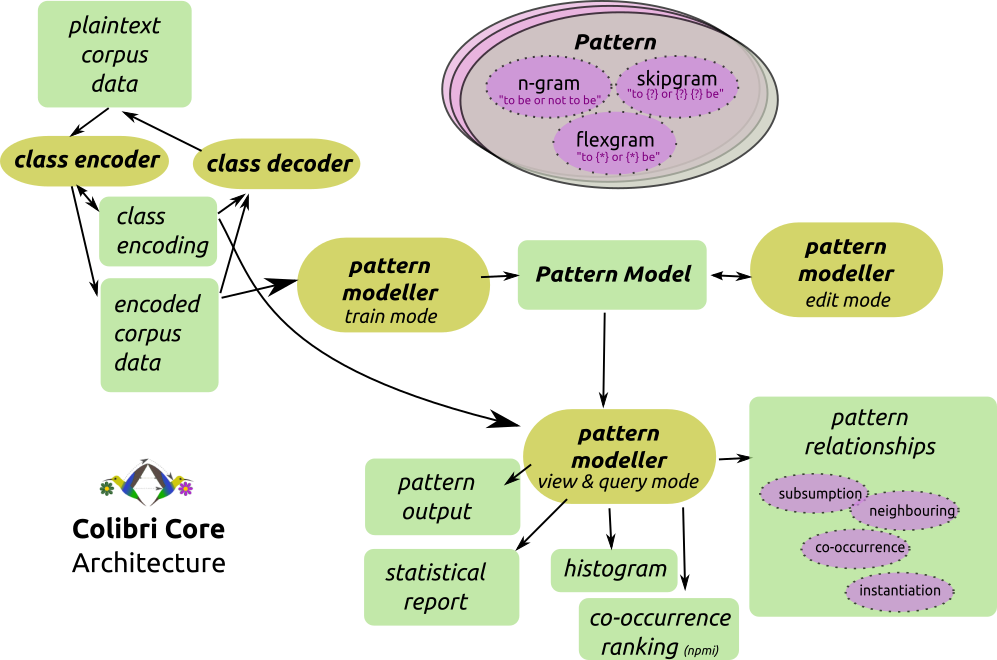
\includegraphics[width=14.0cm]{../cocoarch.png}}
\caption{The Colibri Core architecture; light green squares represent data models, ochre (yellowish) rounded squares represent processes that manipulate data.}
\label{fig:architecture}
\end{figure}

We will present the various features and optimisations that are implemented in
Colibri Core. We start with a introduction of patterns and their encoding, then
discuss the implemented optimisation we use to count n-grams, and subsequently
skipgrams. We then discuss more advanced parametrisation and end with a section
on the computation of flexgrams.

\subsection*{Feature: Patterns}
\label{sec:patterns}

We distinguish three categories of patterns, and define them as follows:

\begin{enumerate}
    \item N-grams -- A sequence of $n$ word tokens that are all consecutive.
        For example: ``\texttt{to be or not to be}''
    \item Skipgrams -- A fixed-length sequence of $p$ word tokens and $q$ token
        placeholders/wildcards with total length $n$ ($n=p+q$), the
        placeholders constitute gaps, or skips, and a skipgram can contain
        multiple of these. In turn, a gap can span one or more tokens. For
    example: ``\texttt{to \_ or \_ \_ be}''
    \item Flexgrams -- A sequence with one or more gaps of variable length,
        which implies the pattern by itself is of undefined length. For example:
        ``\texttt{to * or * be}''
\end{enumerate}

Our definitions are defined narrowly and, with exception of $n$-grams do not
necessarily match up precisely to the way the concepts are used in other studies. Some
may use the term skipgram to include what we call flexgram, or use another term
such as ``elastigram'' to refer to flexgrams \citep{ForsythS14}.

Skipgrams are used in the field to obtain a higher level of generalisation than
can be offered by n-grams. They can, for instance, be found as features in
classification tasks \citep{DHONDT}, or as a means in language modelling to
decrease perplexity \citep{Guthrie06,COCOCPYP}.

Dealing with word tokens implies that the corpus data has to be in a
tokenised form. We start from the basis of plain-text corpus data, containing one
\emph{unit} per line; a unit can correspond to a sentence, paragraph, tweet
or whatever unit is deemed appropriate for the task at hand. Corpus data can
alternatively be provided in FoLiA XML format \citep{FOLIAPAPER} as well, although linguistic
annotation will be ignored.

Text data is typically stored as a string of characters. The characters
themselves draw their denotation from a character encoding. The storage of a
huge amount of strings is inefficient from a memory perspective, considering
the fact that words follow a Zipfian distribution. Colibri Core therefore works
on the basis of a lossless compression, in which each unique word token is
assigned a numeric type identifier, which we call a \emph{class}. This
effectively defines the \emph{vocabulary} of your data, which we call a
\emph{class encoding}. A pattern is not represented as an array of
characters, but as an array of these classes instead. Such methods are commonly
employed in Language Modelling toolkits as well, where 24 or 32-bit integers
uniquely assigned to words are typically chosen \citep{Guthrie2010}.

In Colibri Core, further lossless compression is achieved by holding this array of
classes in a dynamic-length byte representation rather than fixed-sized
integers. This allows  for low class values to be stored in fewer bytes than
high class values. Classes $0$ to $127$ can be stored in a single byte, higher
classes require at least two bytes. To achieve maximum compression, classes are
assigned to word tokens based on frequency (i.e.\ entropy encoding): words with
the highest frequency receive the lowest classes.  This is essentially a
variant of Huffman coding \citep{HUFFMAN}. Some of the lowest classes are
reserved for special purposes, e.g. to delimit sentences (class 0) or as
markers for out-of-vocabulary words (class 2) or skipped content (classes 3 and
4).

Of each byte in the class representation, the highest bit is reserved as a continuation
marker. As long as the continuation marker is set, the next byte is still part of
the class. When it is low, we know we are at the final byte of a class
representation. The class itself is stored in the remaining 7-bits of each
byte. In practise this results in good compression and reduces memory usage; an
example corpus taking up $221$ MB on disk in plaintext form is reduced to just $60$ MB
when compressed. A subset of the Google billion word corpus, 769 million words
in 30 million sentences, takes $3.9$ GB in plaintext form, and $1.2$ GB when
compressed in this matter.

To encode a text corpus, a class encoding needs to be computed first, as
visualised in the top-left corner of Figure~\ref{fig:architecture}. To decode
the encoded corpus back to plain text, the class encoding is needed again.
Colibri Core provides tools and exposes library functions to do this.

\subsection*{Optimisation: Informed Iterative Counting}
\label{sec:iterativecounting}

N-gram frequency lists are often parametrised by a certain threshold. All
$n$-grams below this occurrence threshold are pruned. We can circumvent the
problem of having to hold a huge amount of patterns in memory that do not meet
the threshold, as is typical in a Zipfian distribution. We do this by employing
informed counting. Informed counting is an iterative procedure, shown in pseudo
code in Algorithm~\ref{alg:ngramcounting}. Here we take $m$ to be the maximum
$n$-gram order we intend to extract. The whole corpus is then processed for
each $n$ where $1<n\leq m$, extracting the respective $n$-grams at each
iteration. This means that at each iteration, we can consult the results of the
previous iteration. We can then readily discard any $n$-gram with $n>1$ for
which either of the two $n-1$-grams it contains does not
meet the threshold, as it follows that the $n$-gram can never meet the
threshold either. By outright discarding an $n$-gram we do not need to store it
and its count in memory. After each iteration of $n$, we prune all the
$n$-grams that did not reach the threshold.


\begin{algorithm} \caption{Informed Iterative Counting for n-grams.  Take $m$
to be the maximum $n$-gram order we intend to extract, $t$ to be the minimum occurrence threshold, and $M$ to be the
pattern model in memory, with unigrams already counted in the more trivial fashion.}
\label{alg:ngramcounting}
\begin{algorithmic}
\For {$n \in 2..m$}
    \For {$line \in corpus$}
        \For {$ngram \in extractNGrams(line,n)$}
            \State  $nm1gram_1, nm1gram_2 \leftarrow extractNGrams(ngram,n-1)$
            \If {$M(nm1gram_1) \geq t$ \& $M(nm1gram_2) \geq t$}
                \State $M(ngram) \leftarrow M(ngram) + 1$
            \EndIf
        \EndFor
    \EndFor
    \State $M \leftarrow pruneNGrams(M,n,t)$
\EndFor \\
\Return{M}
\end{algorithmic}
\end{algorithm}

Though not expressed in the simplified algorithm shown in Algorithm~\ref{alg:ngramcounting}, the actual
implementation accounts for more parameters, such as setting a lower bound to
$n$. The amount of back-off, going all the way up to $m-1$ here, can also be
fine-tuned.

This algorithm makes concessions to processing speed, as multiple passes over
the data are needed, to conserve memory. A performance evaluation of this
algorithm will be addressed later in the section on \emph{Quality Control}.

\subsection*{Optimisation: Informed Skipgram Counting}
\label{sec:skipgramcount}

The computation of skipgrams is parametrised by an upper limit $l\leq m$ in the number of
tokens, i.e. the total length of the skipgram (including gaps) expressed in tokens. The possible configuration of gaps
increases exponentially with the total length spanned. A skipgram of size three has only one possible
gap configuration\footnote{The initial and final token may never be gaps in the extracted skipgrams.};
\texttt{a \_ z}, a skipgram of size four already has three possible configurations;
\texttt{a \_ \_ z}, \texttt{a b \_ z} or \texttt{a \_ y z}.

The algorithm, shown in Algorithm~\ref{alg:skipgramcount} considers all
possible configurations in which skips can be inserted in all of the n-grams in the model. It can
discard a skipgram candidate by looking at the non-skipped parts that make up
the skipgram, and by checking whether those exceed the set threshold. Note that
the computation of skipgrams first requires counts of all $n$-grams where
$0<n\geq l$.

\begin{algorithm} \caption{Informed Counting for skipgrams.  Take $l$
to be the maximum skipgram order we intend to extract, $t$ to be the minimum occurrence threshold, and $M$ to be the
pattern model in memory, with ngrams already counted.}
\label{alg:skipgramcount}
\begin{algorithmic}
\For {$n \in 3..l$}
    \For {$ngram \in getNGrams(M,n,t)$}
        \For {$skipgram \in possibleConfigurations(ngram)$}
            \State $docount \leftarrow True$
            \For {$part \in parts(skipgram)$}
            \If {$M(part) < t$}
                    \State $docount \leftarrow False$
                    Break
                \EndIf
            \EndFor
            \If {$docount$}
                \State $M(skipgram) \leftarrow M(skipgram) + 1$
            \EndIf
            \EndFor
            \EndFor
    \State $M \leftarrow pruneSkipgrams(M,n,t)$
\EndFor \\
\Return{M}
\end{algorithmic}
\end{algorithm}

In this algorithm, the $possibleConfigurations(ngram)$ function returns
all possible skipgram configurations for the given $n$-gram. Note that
the configuration of gaps depends only on the length of the $n$-gram, regardless
of its content, and can therefore easily be pre-computed. The
$parts(skipgram)$ function returns all consecutive parts that are
subsumed in the skipgram, i.e.\ the parts delimited by the gaps.

Like Algorithm~\ref{alg:ngramcounting}, Algorithm~\ref{alg:skipgramcount}
assumes a threshold $t>1$. When $t=1$, more trivial algorithms are
invoked, as the user does not want to prune anything. These make only a single
pass over the data. For skipgrams this leads to an explosion of
resulting patterns, exponential with number of tokens, and is best avoided.

\subsubsection{Parametrisation: What counts?}
\label{sec:whatcounts}

The counting algorithms are parametrised by various other parameters which
are not shown in Algorithm~\ref{alg:ngramcounting} and
Algorithm~\ref{alg:skipgramcount} to reduce complexity. The wide variety of
parameters allow the user to influence precisely what is counted and this is one
of the main assets of Colibri Core. Parameters exist to affect the following:

\begin{itemize}
    \item The minimum and maximum length (in words/tokens) of the n-grams
        and/or skipgrams to be extracted. Setting minimum and maximum length to
        the same value will produce a model of homogeneous pattern length
        (e.g.\ only trigrams or words).
    \item A secondary \emph{word} occurrence threshold can be configured. This is a value set higher than
        the primary occurrence threshold. Only patterns
        occurring above the primary threshold, and for which each of the
        individual words/unigrams in the pattern passes the secondary threshold as well, will
        be included in the model.
    \item N-grams that are not subsumed by higher order n-grams, i.e.\ which do
        not  occur as part of a higher order n-gram in the data/model, can be pruned
        from the model. This allows you to extract for instance all trigrams
        and all bigrams and unigrams that make up the trigrams, but not the
        bigrams and unigrams that are not subsumed in trigrams.
    \item Skipgrams can be constrained using the \emph{skip type threshold}. This
        requires that at least the specified number of distinct patterns must fit in the
        gaps of the skipgram. Higher values will produce less skipgrams, but
        typically more generic ones. For instance, a skipgram such as \emph{The \_ house} will
        then only be included in the model if the corpus has instances in which
        the gap can be
        filled by at least the specified number of distinct patterns.
        If the threshold is set to 2 for example, and the corpus contains \emph{The
            big house} and \emph{The small house}, then the skipgram \emph{The
        \_ house} is included. If the corpus only has
        one of these instantiations, and no other instantiations of the
        skipgram either, then the skipgram would not be included.
    \item Skipgrams and n-grams are typically computed using the same
        occurrence threshold, but it is also possible to use a different threshold
        for skipgrams.
\end{itemize}

\subsection*{Feature: Pattern Models}
\label{sec:patternmodels}

A pattern model is a $key \mapsto value$ store, where the keys correspond to
patterns and the values typically correspond to occurrence counts, although any
kind of other value is supported too. Our aim with pattern models is to have a
data structure that allows for \emph{quick} lookup and iteration, as well as
quick insertion during training. Moreover, memory consumption should be as
conservative as possible, to allow handling of big data.

The underlying C++ library allows for choosing the actual underlying container
implementation and value type through \emph{templating}. The default container
datatype is a hash map\footnote{using the \texttt{unordered\_map} STL container
in C++11.}, which guarantees $O(1)$ access and update times under ideal hashing
conditions. The hash\footnote{Spooky Hash v2 is used for hashing:
\url{http://burtleburtle.net/bob/hash/spooky.html}} is computed directly from the
binary representation of a pattern. Storing each pattern individually results
in a lot of redundant information to be stored, as patterns overlap to a large
degree. To conserve memory, the models can store pattern pointers\footnote{Each
pattern pointer takes up 16 bytes.} instead. Instead of duplicating the content
for each pattern, these point to the original corpus data which is held in
memory.

The use of hash maps can be contrasted to the use of suffix (or prefix) tries
\citep{Weiner73}, a common datastructure for storing n-grams in which a tree is
constructed and any path in the tree, complete or incomplete, corresponds to a
suffix (or prefix).  Although suffix tries also benefit from decreased memory
use due to no overlap in pattern data, the strongly linked nature of tries
causes a significant overhead in memory use\footnote{Each pointer consumes 8
    bytes on 64-bit architectures, and one would be needed for every transition
between two tokens.} that quickly exceeds the memory footprint of hash maps.
For this reason, hash maps are the default and tries are currently not
implemented in Colibi Core. The templating, however, does allow for such an
implementation to be added in the future. This flexibility to abstract over the
underlying data structure is one of the assets of Colibri Core.

At this point, we need to address suffix arrays \citep{Manber90} as well, which
is a sorted array of suffixes, derived from suffix tries but with significantly
decreased space requirements. Suffix arrays with longest common prefix (LCP)
arrays will consume less memory than our hash maps, but are typically much
slower to construct and query. Though no exhaustive experiment was conducted to
this end, we did compare a predecessor of Colibri Core with a suffix array
implementation \citep{Stehouwer10} and found our implementation to be
significantly faster in model construction.

We distinguish two types of pattern model, depending on the type of the values,
which in the underlying C++ implementation is subject to templating as well:

\begin{enumerate}
 \item \textbf{Unindexed Pattern Models} -- Values are simple integers
 \item \textbf{Indexed Pattern Models} -- Values are arrays of indices where
     the pattern's occurrences in the corpus are stored.
\end{enumerate}

Obviously, indexed pattern models make a considerably higher demand on memory.
They do, however, allow for a broader range of computations, as shall become
apparent in subsequent sections.

The command-line tool \texttt{colibri-patternmodeller} exposes most of the
functionality for training, viewing and editing pattern models (see also
Figure~\ref{fig:architecture}). In the C++ and Python APIs, this functionality is
generally available through methods on some flavour of the PatternModel class.

\subsection*{Optimisation: Two-step training}

Training indexed patterns models is more memory intensive than training
unindexed models, especially in very large corpora (say at least a hundred
million words). To lower the demand on memory for such corpora, we implement a
\emph{two-step training} procedure. This involves first constructing an
unindexed pattern model and subsequently constructing an indexed model on the
basis of that, by making another pass over the corpus and gathering all
indices. The gain here is in avoiding temporary storage of the indices that
will not pass the occurrence threshold but that cannot be ruled out a priori by the
informed counting algorithm.  This conservation of memory comes at the cost of
extended execution time.

\subsection*{Feature: Corpus Comparison}

The computation of pattern models on two or more distinct corpora, provided the
class encoding is the same for all of them, provides a basis for comparative
corpus analysis. One measure for corpus comparison introduced in the software
is the notion of \emph{coverage}. This metric is expressed as the number of
tokens in the test corpus that is covered by the patterns from the training
corpus. This makes it an asymmetric metric, so the choice of training and test corpus
matters.  The metric can be represented either in absolute counts, or in
normalised form as a fraction of the total amount of tokens in the test corpus.

To perform such comparisons, we first compute a pattern model on the training
corpus, and subsequently compute a second pattern model on the test corpus, but
\emph{constrained} by the former pattern model. The ability to train
constrained models is present throughout the software and can for instance also
be used to train a pattern model based on a custom preset list of patterns,
effectively limiting the model to this preselection. The previously described
two-step training algorithm is also an example of constrained training.

Summarised statistics are computed at multiple levels. Measures such as
occurrence count and coverage can be consulted for aggregates of n-grams,
skipgrams, or flexgrams, as well as specific patterns. The former two can be
inspected specifically for each of the different pattern sizes present in the
model, i.e.\ for each value of $n$.

The coverage metric is a fairly crude metric of corpus overlap, despite the
ability to assess it for different aggregates. A more widely established metric
for corpus comparison is \emph{log-likelihood}. Log likelihood expresses how
much more likely any given pattern is for either of the two models. It
therefore allows you to identify how indicative a pattern is for a particular
corpus. Our implementation follows the methodology
of~\cite{Rayson00comparingcorpora}. They compute the log-likelihood ($L$)
given the frequency of a pattern in corpus 1 ($a$), and corpus 2 ($b$) as
follows\footnote{Here, $E_i$ expresses expected values, $N_i$ is the
total amount of tokens in the respective corpus.}:

\begin{equation}
L = 2a(\log \frac{a}{E_1}) + b(\log \frac{b}{E_2})\text{, where } E_i = \frac{N_i(a+b)}{N_1 + N_2}
\end{equation}


\subsection*{Feature: Relations between Patterns}

Various relations can be extracted between patterns in a pattern model, either
through the API or a dedicated query tool. For all but the first of the
relation types an indexed pattern model is required.

\begin{itemize}
 \item \textbf{Subsumption Relation} -- $n$-gram $x y z$ subsumes $n-1$-grams $x y$ and $y z$.
 \item \textbf{Succession Relation} -- Patterns that occur in a sequence in the
     corpus data. For example: pattern $x$ precedes $yz$ and pattern $z$ succeeds $xy$.
 \item \textbf{Instantiation Relation} -- Skipgrams or flexgrams may be
     \emph{instantiated} by other patterns. For example, ``to be \_ not \_'' be
     is instantiated by ``or \_ to'', resulting in the 6-gram ``to be or not to be''. This type of relation thus allows you to precisely determine what patterns occur in certain gaps.
 \item \textbf{Co-occurrence Relation} -- Different patterns can naturally co-occur multiple times
     within the the structural ``units'' you decided upon for the corpus (e.g.\
     sentences, paragraphs, tweets, etc). These units are newline delimited in
     your original input. The measure of such co-occurrence
     can be expressed by established metrics such as Jaccard and (normalised) mutual
     pointwise information.
\end{itemize}

For each of these categories, the relationship is bidirectional, i.e.\ you can
query for the subsuming patterns as well as the subsumed patterns, the left
neighbours as well as the right neighbours, the instantiations as well as the
abstractions. The co-occurrence relationship is fully symmetrical.

These latter three relationships rely on both the \emph{forward index} inherent
in an indexed pattern model, as well as the \emph{reverse index}, a function
from positions in the corpus to an array of patterns that are found at said
position. The reverse index is not modelled in memory as an explicit mapping
from positions to patterns, that would use too much memory, but as a simpler
reverse index that only keeps track of where each unit/sentence starts. This
can then be used to quickly resolve specific positions to all possible
patterns.

\subsection*{Feature: Flexgram Counting}

Thus far, we have explained the algorithms for n-gram counting and skipgram
counting, but have not yet done so for flexgrams, i.e. patterns with
variable-width gaps. The implementation allows flexgrams to be computed in two
different ways. The first is by extracting skipgrams first, and then
abstracting flexgrams from these skipgrams. In this case the flexgram
computation is constrained by the same maximum-size limit under which the
skipgrams have been extracted.  The second method for flexgram extraction
proceeds through the co-occurrence relation. A flexgram is formed whenever two
patterns (within the same structural unit) co-occur above a set threshold. The
implementation of this latter method is currently limited to flexgrams with a
single variable-width gap. This method is recommended when the user is
interested in long-distance flexgrams, whereas the abstraction method is
recommended when the user is more interested in having multiple gaps or
the relationship between flexgrams and skipgrams.


\section{Quality Control}
\label{sec:qc}

\subsection*{Unit tests}

To ensure the software is working as intended, an extensive series of unit
tests is available.  The tool \texttt{colibri-test} tests the various functions
of the C++ library. The \texttt{test.py} script tests the Python binding.
Testing in the form of continuous integration is made possible through
\emph{Travis CI}, where all test results are publicly available for inspection.
\footnote{\url{https://travis-ci.org/proycon/colibri-core}}

\subsection*{Performance Evaluation}

In this section we conduct a performance evaluation of Colibri Core by
measuring the time to compute a pattern model, and the memory resources used.

Comparisons can be made between Colibri Core's
unindexed vs indexed models, between the optimised pointer models vs
standard pattern models, and between preloading a corpus in memory or reading
it directly from file.  For the experiments, shown in
Table~\ref{tab:benchmarks}, we used a corpus of Dutch
translations of TED talks of $127,806$ sentences and $2,330,075$
words\footnote{The data is from the IWSLT 2012 Evaluation Campaign,
    \url{http://hltc.cs.ust.hk/iwslt/index.php/evaluation-campaign/ted-task.html\#MTtrack}.
Tokenisation was performed using ucto,
\url{https://languagemachines.github.io/ucto}, version v0.5.3.}.

We perform tests without thresholding as well as with an occurrence threshold
of $2$, and extract anything from unigrams to $8$-grams.

For reference, we include a naive Python implementation that simply counts
n-grams and stores them in a Python dictionary where the keys are strings and
the values integers. We also include a comparable implementation that uses
NLTK\footnote{Natural Language Toolkit, a popular platform for NLP on Python:
    \url{http://www.nltk.org}. Our implementation follows the naive approach
    but uses \texttt{ngrams()} from \texttt{nltk.util} and \texttt{FreqDist} from
\texttt{nltk.probability}. We used version 2.0.4.}. Similarly, we include a naive C++ implementation based on \\
\texttt{std::unordered\_map$<$string,uint32\_t$>$}. The memory reduction that can be
observed when comparing these against the Colibri Core models is attributed to
the class encoding scheme we use. These memory optimisations do come with a
performance drawback that is especially noticeable when no thresholding is
applied.

The pattern pointer models prove capable of further reduction in memory
consumption, and offer a clear speed advantage as well. The pointer models use a
representation of patterns that refer to the original corpus data, which is
fully loaded into memory, rather than storing a separate copy for each pattern.

For the experiments with thresholding, we added a simple Python implementation of
iterative counting and assess the value of the algorithm as such by comparing
it against the naive Python implementation that simply prunes values below
threshold at the very end. We clearly observe a drastic reduction in memory
usage, at the cost of a longer execution time due to the multiple iterations.

Though Colibri Core is not a Language Modelling toolkit in itself, a comparison
with a popular third-party LM toolkit may be of interest. We compare an
unindexed pattern model containing unigrams, bigrams and trigrams to a similar
model in SRILM \citep{SRILM}. \footnote{SRILM's \texttt{ngram-count} is run in
vanilla form, i.e. no smoothing or interpolation, with the options
\texttt{-no-bos -no-eos}. Note that the encoding of classes is a separate step in
Colibri Core, so our total CPU time should be considered to be a second longer
than reported for a more fair comparison.} Due to the many other features
Colibri Core offers regarding thresholding, indexing, skipgrams and flexgrams, it
can not yet rival the performance and memory efficiency of dedicated LM systems,
which allow for more specific optimisations.

\begin{table}[h]
\footnotesize{
\noindent\makebox[\textwidth][c]{%
\begin{tabular}{lll}
Experiment & CPU time & Memory  \\
\hline
\multicolumn{3}{c}{\textbf{IWSLT data, without thresholding} ($t=1,l=8$)} \\
\hline
$\ast$ Naive Python implementation & $20.0$ s & $1404$ MB \\
$\ast$ Python NLTK implementation & $18.7$ s & $1413$ MB \\
$\ast$ Naive C++ implementation  & $10.5$ s & $1398$ MB \\
Unindexed Pattern Model (from file) & $29.7$ s & $775$ MB ($787$ MB) \\
Unindexed Pattern Pointer Model (preloaded corpus) & $19.8$ s & $615$ MB ($627$ MB) \\
\hline
\multicolumn{3}{c}{\textbf{IWSLT data, with thresholding ($t=2,l=8$)}} \\
\hline
$\ast$ Naive Python implementation & $28.8$ s & $1485$ MB \\
$\ast$ Python with iterative counting  & $70.9$ s & $171$ MB \\
Unindexed Pattern Model (from file) & $14.6$ s & $64$ MB ($76$ MB) \\
Unindexed Pattern Model (preloaded corpus) & $11.3$ s & $64$ MB ($76$ MB) \\
Unindexed Pattern Pointer Model (preloaded corpus)  & $9.0$ s & $50$ MB ($62$ MB) \\
Indexed Pattern Model (preloaded corpus) & $13.6$ s & $148$ MB ($160$ MB) \\
Indexed Pattern Pointer Model (preloaded corpus) & $10.1$ s & $133$ MB ($146$ MB) \\
Unindexed Pattern Model (ordered map) & $30.5$ s & $84$ MB ($96$ MB) \\
\hline
Unindexed Pattern Model (preloaded corpus), with skipgrams & $62.4$ s & $105$ MB ($118$ MB) \\
Unindexed Pattern Pointer Model (preloaded), skipgrams  & $50.0$ s & $89$ MB ($102$ MB) \\
Indexed Pattern Model (preloaded corpus), with skipgrams & $24.2$ s & $165$ MB ($178$ MB) \\
\hline
\multicolumn{3}{c}{\textbf{IWSLT data, LM comparison, trigram model ($t=1,l=3$)}} \\
\hline
Unindexed Pattern Model (from file) & $5.9$ s & $152$ MB ($164$ MB) \\
$\ast$ SRILM ngram-count & $1.5$ s & $80$ MB  \\
\end{tabular}}
\caption{Colibri Core performance benchmarks on the IWSLT data set. Performed by the \texttt{colibri-benchmarks} tool and the
\texttt{benchmarks.py} script for the Python baselines. All non-Colibri Core
references are marked with an asterisk ($\ast$). Memory usage is measured as the difference in resident memory after training
and before training. Peak memory usage is measured absolutely as reported by
the OS and included in parentheses. All experiments were performed on a Linux system
with an Intel Xeon CPU (E5-2630L v3) at 1.80GHz and 256GB RAM. Parameter $t$ refers to the occurrence threshold, $l$ to the maximum pattern length.
}
\label{tab:benchmarks}
}
\end{table}

Indexed Pattern Models are by definition larger in memory than unindexed
models, but they do offer a significant speed benefit in the computation of
skipgrams, both of this can be observed in Table~\ref{tab:benchmarks}.

The C++ library allows for easy swapping of the underlying datastructure for
pattern models. The default hashmap \\ (\texttt{std::unordered\_map}) solution can
be contrasted to a pattern model using using an ordered map
(\texttt{std::map}\footnote{the hash key is still computed as it determines the
ordering.}). As expected, the ordered map proves to be significantly slower and
does not yield a memory advantage either.

As Colibri Core is suited for the processing of large data sets, provided sensible
thresholds are set, we conduct extra experiments on the JRC-Acquis corpus,
containing $31.3$ million words in over $850,000$ sentences, and on a portion
of the Google Billion Word corpus, where we use a set of $768$ million words in
$30$ million sentences. These results are shown in Table~\ref{tab:benchmarks2}.

\begin{table}[h]
\footnotesize{
\noindent\makebox[\textwidth][c]{%
\begin{tabular}{lll}
Experiment & CPU time & Memory  \\
\hline
\multicolumn{3}{c}{\textbf{JRC-Acquis data, with thresholding ($t=2,l=8$)}} \\
\hline
$\ast$ Naive Python implementation & 8m 4s & $11407$ MB \\
Unindexed Pattern Model (from file) & 4m 18s & $1704$ MB ($1803$ MB) \\
Unindexed Pattern Model (preloaded corpus) & 3m 58s & $1700$ MB ($1800$ MB) \\
Unindexed Pattern Pointer Model (preloaded corpus) & 3m 1s & $1344$ MB ($1445$ MB) \\
Indexed Pattern Model (preloaded corpus) &  4m 36s & $4117$ MB ($4217$ MB) \\
\hline
Unindexed Pattern Model (preloaded corpus), skipgrams & 61m 1s & $30420$ MB ($30520$ MB) \\
\hline
Indexed Pattern Model (prel.), skipgrams, skiptypes$=12$ & 80m 11s & $29746$ MB ($29846$ MB) \\
\hline
\multicolumn{3}{c}{\textbf{JRC-Acquis data, LM comparison, trigram model ($t=1,l=3$)}} \\
\hline
Unindexed Pattern Model (from file) & 42 s & $716$ MB ($847$ MB) \\
$\ast$ SRILM ngram-count & 12 s & $348$ MB  \\
\hline
\multicolumn{3}{c}{\textbf{Google Billion Words corpus, with heavy thresholding ($t=10,l=4,y=20$)}} \\
\hline
Unindexed Pattern Pointer Model (preloaded corpus) & 83m 14s & $12279$ MB ($15317$ MB) \\
\hline
\multicolumn{3}{c}{\textbf{Google Billion Words corpus, trigram model ($t=1,l=3$)}} \\
\hline
Unindexed Pattern Model (from file) & $25m 16s$ & $16568$ MB ($19788$ MB) \\
\end{tabular}}
\caption{Benchmarks on two large data sets. Same setup as Table~\ref{tab:benchmarks}. Parameter $y$ represents the occurrence threshold specifically for skipgrams.}
\label{tab:benchmarks2}
}
\end{table}

Noticeable in the big data experiments is the explosion in memory consumption
when skipgrams are computed on an unindexed pattern model. This is attributed
directly to the sheer amount of skipgrams that can be extracted from the data,
and the fact that unindexed models can only compute skipgrams exhaustively and
do not support the skip type threshold discussed in Section ``Parametrisation:
What counts?''.

\FloatBarrier

\subsection*{Documentation}

Extensive documentation, including API references for both Python and C++, is provided at
\url{https://proycon.github.io/colibri-core}. An interactive tutorial for Python is also
available. The next section will provide a small example of possible usage from the command line.

\subsection*{Usage Example}

Although we refer to the aforementioned documentation and the Python tutorial
for extensive usage instructions, we include a short use case in this section
and show how to use the command line tools.  Assume you have a corpus
\texttt{corpus.txt} and you want to extract all n-grams, skipgrams and
flexgrams that occur more than five times. We set the maximum length to $8$. For
skipgrams, we add the additional constraint that it abstracts over at least
three distinct ngrams, i.e. there are three different ways of filling the gaps.
Flexgrams we derive from skipgrams.

First we should ensure this corpus is properly tokenised and that sentence
splitting has been performed, putting each sentence on one line to make this
the basic unit Colibri Core can count with. This preprocessing is not done by
Colibri Core but using an external tokeniser such as ucto\footnote{\url{https://languagemachines.github.io/ucto}}:

\begin{verbatim}
$ ucto ucto -L en -n corpus.txt > corpus.tok.txt
\end{verbatim}

Once preprocessing is done, we can encode the corpus in a form suitable for
Colibri Core, computing a \emph{class encoding} and converting the data to it,
as explained in section ``Feature: Patterns''.  The flow of this and all
subsequent steps is also visualised in the architectural scheme in
Figure~\ref{fig:architecture}.

\begin{verbatim}
$ colibri-classencode corpus.tok.txt
\end{verbatim}

This will result in the encoded corpus \texttt{corpus.tok.colibri.dat} and the corresponding vocabulary file \texttt{corpus.tok.colibri.cls}.

The main tool \texttt{colibri-patternmodeller} can now be invoked to extract
ngrams, skipgrams and flexgrams and output a pattern model, as described in
section ``Feature: Pattern models'', to file:

\begin{verbatim}
$ colibri-patternmodeller --datafile corpus.tok.colibri.dat \
--outputmodel corpus.colibri.patternmodel --threshold 5 \
--maxlength 8 --skipgrams --skiptypes 3 --flexgrams S
\end{verbatim}

We have opted for an indexed pattern model, which gives us more thresholding
options such as \texttt{--skiptypes}, and makes skipgram extraction more
efficient, but at the cost of a much higher memory footprint compared to
the simpler unindexed models\footnote{Use the \texttt{--unindexed} flag to
build an unindexed model.}.

We can now read the model from file and produce output to standard output in
the form of \emph{1)} a print of all patterns in the model, \emph{2)} a
statistical report summarising counts for various groups of patterns, and
\emph{3)} a histogram of pattern frequencies:

\begin{verbatim}
$ colibri-patternmodeller \
--inputmodel corpus.colibri.patternmodel \
--classfile corpus.tok.colibri.cls \
--print --report --histogram
\end{verbatim}

This step could have been combined with the previous one as well.

We again urge the reader to consult the documentation and tutorials for a more
extensive description of all available options and use cases, as this example
only covers one out of many use cases, and further in-depth examples fall beyond
the scope of this paper.

\subsection*{Support}

Support, including but not limited to bug reports, feature requests and general
pleas for assistance, is provided through the Github issue tracker at
\url{https://github.com/proycon/colibri-core/issues}. As such, the archive of
issues is always publicly consultable.

\section{Availability}

\subsection*{Operating System}

Colibri Core should be able to run on modern POSIX-compliant operating systems, including
Linux, FreeBSD and Mac OS X. It is tested to compile with current versions of
both \texttt{gcc} as well as \texttt{clang}.

\subsection*{Programming Language}

Colibri Core is written in C++, adhering to the C++11 standard. The Python
binding is written in Cython (0.23 or above) and supports both Python 2.7 as
well as Python 3. The latter is recommended.

The Python binding ensures that the functionality of Colibri Core is easily
accessible from Python without sacrificing the great performance benefit native
code provides. Python was chosen as it is a high-level programming language in
widespread use in the scientific community, and the NLP community in
particular. It demands less expertise from the developer than C++ and is more
suitable for rapid prototyping.

\subsection*{Additional system requirements}

Colibri Core provides memory-based techniques where models are held entirely in
memory to guarantee maximum performance on lookup and computation.  This
approach can be contrasted to e.g.\ database approaches which have much higher
latency.  It does place considerable memory requirements on the system on which
is it run, though this depends entirely on the size of the data and the
thresholds the user uses. We recommend at least 16GB RAM. In practise, using Colibri
Core on high-end computing servers with 256GB RAM is not uncommon for extensive
computation on big data sets.

Colibri Core is single-threaded due to the non-distributable nature of most of the
algorithms. A 64-bit architecture is required, 32-bit is not supported.

\subsection*{Dependencies}

Colibri Core relies on the standard C/C++ library and a full build environment including autoconf and
automake; Python 2.7 or 3; Cython 0.23 or above. Support for reading the
\emph{FoLiA} XML format for text is entirely optional and requires the \texttt{libfolia}
library.\footnote{\url{https://proycon.github.io/folia}}

\subsection*{List of contributors}

Developed by Maarten van Gompel, with contributions and feedback from Louis
Onrust and Antal van den Bosch (\emph{Centre for Language Studies, Radboud
University Nijmegen}).

\subsection*{Software Location}

\subsubsection*{Archive}

%\begin{addmargin}[2em]{2em}
\textbf{Name}: Zenodo \\
\textbf{Persistent Identifier}: \url{https://dx.doi.org/10.5281/zenodo.55641} \\
\textbf{Publisher}: Maarten van Gompel \\
\textbf{Licence}: GNU General Public Licence v3 \\
\textbf{Date published}: June 15th, 2016 (v2.4.1) \\
%\end{addmargin}

\subsubsection*{Code repository}

%\begin{addmargin}[2em]{2em}
\textbf{Name}: GitHub \\
\textbf{Identifier}: \url{https://github.com/proycon/colibri-core} \\
\textbf{Website}: \url{https://proycon.github.io/colibri-core} \\
\textbf{Licence}: GNU General Public Licence v3 \\
\textbf{Date published}: since September 21st, 2013, latest release at the time
of writing is v2.4.1 (June 15th, 2016) \\
%\end{addmargin}

\subsection*{Language}

English

\section{Reuse potential}

Colibri Core explicitly aims to provide a foundation for researchers in the NLP
community to build their tools and research on. The software is already being
employed in ongoing research on Machine
Translation\footnote{\url{https://github.com/proycon/colibri-mt}}, Bayesian Language
Modelling\footnote{\url{https://github.com/naiaden/cococpyp}}, Kneser-Ney Language
Modelling\footnote{\url{https://github.com/naiaden/apodiformes}}, spelling
correction\footnote{\url{https://github.com/proycon/gecco}}, and event
prediction in social media streams\footnote{\url{https://github.com/fkunneman/ADNEXT\_predict}}.
This has culminated in the publication of several studies that use Colibri Core
\citep{COLIBRITAPILOT,COCOCPYP,Kunneman+16}.

As a programming library for both C++ and Python, Colibri Core can be
potentially adopted by a wide variety of third party developers. As a set of
tools and scripts, Colibri Core also has merit standalone. It is, however,
focused on command-line usage and therefore still requires a certain technical
expertise from the end-user.

To increase the accessibility of Colibri Core, a RESTful webservice as well as
generic web interface is already provided through CLAM \citep{CLAMPAPER}. With this we
hope to meet the needs of less technical end-users, as well as automated
networked clients. This webservice is hosted at
\url{https://webservices-lst.science.ru.nl}.

Future work building upon Colibri Core may focus on offering
high-level user-interfaces to reach a wider audience, and on further
improvement of its performance.

